% Build with: xelatex report.tex
\documentclass[11pt,a4paper]{article}

\usepackage[margin=2.5cm]{geometry}
\usepackage{fontspec}
\usepackage{xeCJK}
\usepackage{graphicx}
\usepackage{booktabs}
\usepackage{xcolor}
\usepackage{tikz}
\usepackage[most]{tcolorbox}
\usepackage{enumitem}
\usepackage{caption}
\usepackage{float}
\usepackage[hidelinks]{hyperref}

\setmainfont{IBM Plex Serif}
\setsansfont{IBM Plex Sans}
\setmonofont{IBM Plex Mono}[Scale=0.9]
\setCJKmainfont{Noto Serif CJK JP}
\setCJKsansfont{Noto Sans CJK JP}
\setCJKmonofont{Noto Sans Mono CJK JP}[Scale=0.9]

\definecolor{fr}{HTML}{2A78D6}
\definecolor{ja}{HTML}{EB6834}
\definecolor{ink}{HTML}{0B0B0B}
\definecolor{muted}{HTML}{52514E}
\definecolor{line}{HTML}{E4E3DF}
\definecolor{unk}{HTML}{8A8985}

\captionsetup{font=small,labelfont=bf}
\setlist{itemsep=2pt}

% Token boxes: \tokens[fr]{je|suis|un|chat} draws one box per token.
% UNK is drawn as a grey [UNK] box.
\newtcbox{\tokbox}[1][fr]{on line, nobeforeafter, boxsep=0pt, left=3pt, right=3pt,
  top=2pt, bottom=2pt, arc=2pt, boxrule=0.5pt, colframe=#1, colback=#1!8,
  fontupper=\ttfamily\small}
\newtcbox{\unkbox}{on line, nobeforeafter, boxsep=0pt, left=3pt, right=3pt,
  top=2pt, bottom=2pt, arc=2pt, boxrule=0.5pt, colframe=unk, colback=unk!12,
  fontupper=\ttfamily\small\color{muted}}
\ExplSyntaxOn
\NewDocumentCommand\tokens{ O{fr} m }
  {
    \seq_set_split:Nnn \l_tmpa_seq { | } { #2 }
    \seq_map_inline:Nn \l_tmpa_seq
      {
        \str_if_eq:nnTF { ##1 } { UNK }
          { \unkbox{[UNK]} }
          { \tokbox[#1]{##1} }
        \hspace{2pt~plus~1pt}\allowbreak
      }
  }
\ExplSyntaxOff
% The "▁" that SentencePiece puts in front of a word.
\newcommand\wsp{\rule[-0.1ex]{0.45em}{0.5pt}}

\newcommand\code[1]{\texttt{#1}}
\newenvironment{result}
  {\par\smallskip\noindent\begin{tabular}{@{}l p{0.78\textwidth}@{}}}
  {\end{tabular}\par\smallskip}
\newcommand\row[2]{\textsf{\small\color{muted}#1} & #2 \\[3pt]}

\begin{document}

% ---------------------------------------------------------------- cover
\begin{titlepage}
\setlength{\parindent}{0pt}
\begin{tikzpicture}[remember picture, overlay]
  \fill[fr] (current page.north west) rectangle ([yshift=-0.9cm]current page.north east);
  \fill[ja] ([yshift=-0.9cm]current page.north west) rectangle ([yshift=-1.3cm]current page.north east);
\end{tikzpicture}

\vspace*{3.5cm}
{\sffamily\color{muted}\large Natural Language Processing}

\vspace{0.6cm}
{\sffamily\bfseries\fontsize{34}{40}\selectfont\color{ink} Tokenization:\\[4pt] French vs Japanese\par}

\vspace{0.6cm}
{\large\color{muted} How splitting text into words works when a language\\ does not use spaces\par}

\vspace{2.8cm}
\begin{tabular}{@{}l l@{}}
  \textsf{\small\color{muted}French} & \tokens[fr]{je|suis|un|chat} \\[10pt]
  \textsf{\small\color{muted}Japanese, split on spaces} & \tokens[ja]{吾輩は猫である} \\[10pt]
  \textsf{\small\color{muted}Japanese, MeCab} & \tokens[ja]{吾輩|は|猫|で|ある} \\
\end{tabular}

\vfill
\noindent\textcolor{line}{\rule{\textwidth}{0.6pt}}\par\smallskip
\noindent{\sffamily Joah Emy-Nakane \hfill October 2026}
\end{titlepage}

% ---------------------------------------------------------------- body
\section{Introduction}

Before a model can read text, the text has to be cut into \emph{tokens}, and
every token gets an integer id from a vocabulary. In French, the obvious way is
to cut on spaces. Japanese does not put spaces between words, so that rule does
not work.

This report compares the two languages in three steps:
\begin{enumerate}
  \item a toy corpus of five sentences, passed through
        \code{keras.layers.TextVectorization}, the layer used in the course
        notebook;
  \item a real corpus of 38{,}292 French--Japanese sentence pairs from
        Tatoeba, with the Japanese side split by the morphological analyzer
        MeCab;
  \item the same pairs passed through two multilingual subword tokenizers.
\end{enumerate}
All the code is in the repository: \code{french/}, \code{japanese/} and
\code{corpus/}.

% ----------------------------------------------------------------
\section{A toy example}

Both corpora contain five short sentences. The vocabulary is built from the
corpus with \code{adapt()}, then a test sentence that is not in the corpus is
encoded and decoded.

\subsection{French}

By default, \code{TextVectorization} lowercases the text, strips punctuation
and splits on whitespace. In French, that directly gives words.

\begin{result}
  \row{Vocabulary}{\tokens[fr]{UNK|je|un|suis|texte|écrivain|écrire|si|sait|pense|pas|ne|chat|autre}}
  \row{Sentence}{Je suis un chat qui sait écrire}
  \row{Encoded}{\code{[2, 4, 3, 13, 1, 9, 7]}}
  \row{Decoded}{\tokens[fr]{je|suis|un|chat|UNK|sait|écrire}}
\end{result}

Only \emph{qui}, which is not in the corpus, becomes \code{[UNK]}. (Index 0 is
kept for padding and index 1 for \code{[UNK]}.)

\subsection{Japanese, split on spaces}

With the same settings, each Japanese sentence is a single token, because it
contains no space:

\begin{result}
  \row{Vocabulary}{\tokens[ja]{UNK|私は猫ではありません|私は別のテキストです|私はテキストです|我思う、ゆえに我あり|作家は書くことができる}}
  \row{Sentence}{私は書くことができる猫です}
  \row{Encoded}{\code{[1]}}
  \row{Decoded}{\tokens[ja]{UNK}}
\end{result}

The test sentence never appears as-is in the corpus, so the whole sentence is
unknown, even though it reuses known pieces: 私は (\emph{I}), 書くことができる
(\emph{can write}) and 猫 (\emph{cat}).

\subsection{Japanese, split by character}

With \code{split="character"}, every character is a token:

\begin{result}
  \row{Vocabulary}{\tokens[ja]{UNK|は|で|私|我|ト|テ|ス|キ|り|す|あ|猫|書|思|家|別|作|ん|る|ゆ|ま|の|に|と|せ|こ|く|き|が|え|う|、}}
  \row{Encoded}{\code{[4, 2, 14, 28, 27, 25, 30, 3, 29, 20, 13, 3, 11]}}
  \row{Decoded}{\tokens[ja]{私|は|書|く|こ|と|が|で|き|る|猫|で|す}}
\end{result}

There is no \code{[UNK]} any more, but the notion of a word is gone: テキスト
(\emph{text}) is split into four characters. Note also that 、 stays in the
vocabulary: the default standardization only strips ASCII punctuation.

\subsection{Japanese with MeCab}

MeCab is a morphological analyzer. It uses a dictionary (here UniDic, installed
with \code{unidic-lite}) to cut the text into words and tag each one with its
part of speech:

\begin{center}
\begin{tabular}{l l l}
  \toprule
  Token & Tag & \\
  \midrule
  私 & 代名詞 & pronoun \\
  は & 助詞 & particle \\
  書く & 動詞 & verb \\
  こと & 名詞 & noun \\
  が & 助詞 & particle \\
  できる & 動詞 & verb \\
  猫 & 名詞 & noun \\
  です & 助動詞 & auxiliary verb \\
  \bottomrule
\end{tabular}
\end{center}

With the \code{-Owakati} option, MeCab only outputs the words separated by
spaces. That text can then go through \code{TextVectorization} with the default
settings, exactly like French:

\begin{result}
  \row{Vocabulary}{\tokens[ja]{UNK|は|私|我|テキスト|です|あり|猫|書く|思う|別|作家|ん|ゆえ|ませ|の|に|できる|で|こと|が|、}}
  \row{Sentence}{私 は 書く こと が できる 猫 です}
  \row{Encoded}{\code{[3, 2, 9, 20, 21, 18, 8, 6]}}
  \row{Decoded}{\tokens[ja]{私|は|書く|こと|が|できる|猫|です}}
\end{result}

No \code{[UNK]}, and the tokens are words again: テキスト stays in one piece,
書く (\emph{to write}) and 猫 (\emph{cat}) are recognized.

\subsection{Summary}

\begin{table}[H]
\centering
\begin{tabular}{l r r l}
  \toprule
  Method on 私は書くことができる猫です & Tokens & \code{[UNK]} & Tokens are \\
  \midrule
  Whitespace split & 1 & 1 & whole sentences \\
  Character split & 13 & 0 & single characters \\
  MeCab, then whitespace split & 8 & 0 & words \\
  \bottomrule
\end{tabular}
\end{table}

Five sentences are enough to see that Japanese needs an extra step before the
usual pipeline. They are not enough to say how the result compares to French
on real text.

% ----------------------------------------------------------------
\section{A real corpus: Tatoeba}

\subsection{Setup}

Tatoeba (\url{https://tatoeba.org}) is a collection of sentences translated by
volunteers. Its exports give 43{,}856 links between a French and a Japanese
sentence. When a sentence has several translations, only one pair is kept, so
both sides have the same number of distinct sentences: \textbf{38{,}292 pairs},
shuffled and split into 30{,}633 for training and 7{,}659 for testing. The
sentences are short and everyday:

\begin{result}
  \row{French}{Nous nous sommes dépêchés pour attraper le bus.}
  \row{Japanese}{私たちはバスに乗るために急いだ。}
\end{result}

Because the content is the same on both sides, the differences come from the
languages and from how they are split, not from the topics.

\begin{itemize}
  \item French is split on whitespace, as \code{TextVectorization} does by
        default.
  \item Japanese is first split by MeCab (\code{-Owakati}), then on whitespace.
  \item In both languages, the text is lowercased and \emph{all} punctuation
        and symbols are removed (regex \code{[\textbackslash p\{P\}\textbackslash p\{S\}]}),
        so that 。 and 、 are not counted as Japanese words.
\end{itemize}

The script is \code{corpus/compare.py}.

\subsection{Sentence length}

\begin{table}[H]
\centering
\begin{tabular}{l r r r}
  \toprule
  Mean per sentence & Characters & Tokens & Characters per token \\
  \midrule
  \textcolor{fr}{French} & 33.7 & 7.6 & 4.45 \\
  \textcolor{ja}{Japanese} & 15.6 & 9.8 & 1.60 \\
  \bottomrule
\end{tabular}
\end{table}

Japanese says the same thing with half as many characters, because a kanji
carries a lot of meaning (急 alone means \emph{hurry}). But it needs
\emph{more} tokens: MeCab cuts out every particle and every auxiliary, which
French either does not have or glues to the word.

\subsection{Vocabulary growth}

\begin{figure}[H]
  \centering
  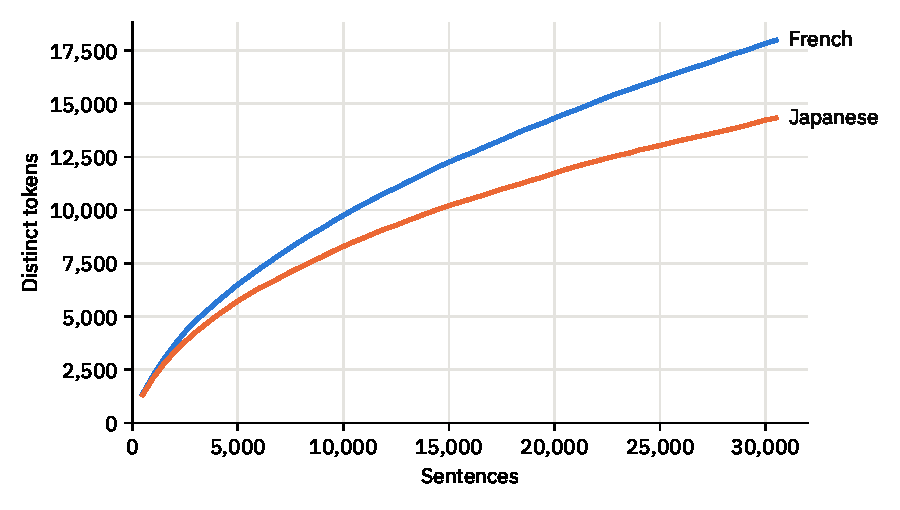
\includegraphics[width=0.7\textwidth]{figures/vocabulary_growth.pdf}
  \caption{Number of distinct tokens as sentences are added (training set).}
\end{figure}

On the 30{,}633 training sentences, French ends with \textbf{18{,}025} distinct
tokens and Japanese with \textbf{14{,}362}. Half of them are seen only once
(52\,\% in French, 47\,\% in Japanese). Both curves keep rising, but the
French one rises faster: every verb has many surface forms (\emph{écris},
\emph{écrit}, \emph{écrivons}, \emph{écrivait}…), each one a different token.
In Japanese, MeCab separates part of the conjugation into its own tokens
(急い + だ), so the same pieces come back more often.

\subsection{Unknown tokens}

A model has a fixed vocabulary (\code{max\_tokens}). The vocabulary is built on
the training set, then we count how many tokens of the test set fall outside
of it.

\begin{figure}[H]
  \centering
  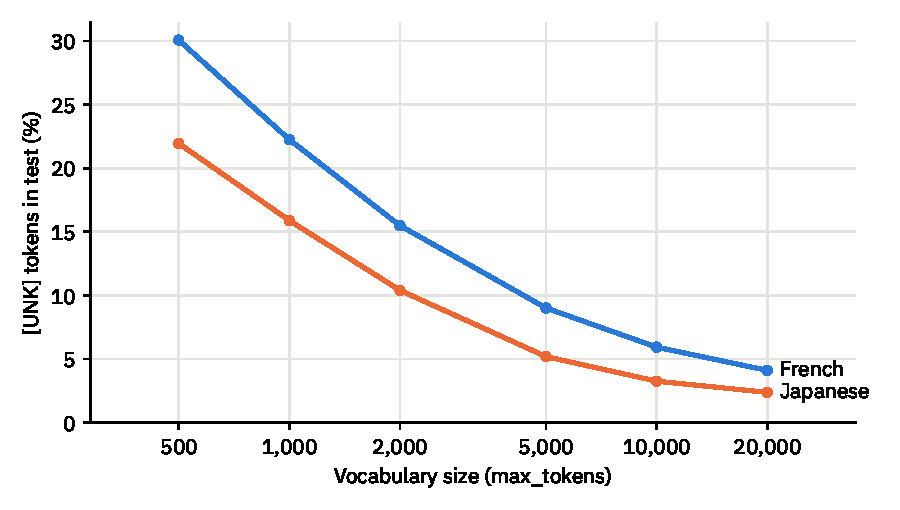
\includegraphics[width=0.7\textwidth]{figures/unk_rate.pdf}
  \caption{Share of \code{[UNK]} tokens in the test set, for a given
  vocabulary size.}
\end{figure}

\begin{table}[H]
\centering
\begin{tabular}{l r r r r r r}
  \toprule
  \code{max\_tokens} & 500 & 1{,}000 & 2{,}000 & 5{,}000 & 10{,}000 & 20{,}000 \\
  \midrule
  \textcolor{fr}{French} & 30.1\,\% & 22.3\,\% & 15.5\,\% & 9.0\,\% & 5.9\,\% & 4.1\,\% \\
  \textcolor{ja}{Japanese} & 21.9\,\% & 15.9\,\% & 10.4\,\% & 5.2\,\% & 3.3\,\% & 2.4\,\% \\
  \bottomrule
\end{tabular}
\end{table}

For every vocabulary size, Japanese split by MeCab has fewer unknown tokens
than French split on spaces. With 5{,}000 tokens, 9\,\% of French tokens are
unknown against 5.2\,\% in Japanese. Once MeCab has done its job, Japanese is
not harder to cover than French; on this corpus it is even easier.

\subsection{What spaces miss in French}

Spaces are not perfect either. When the punctuation is removed, an apostrophe
or a hyphen glues two words into one token. On this corpus, that gives
\textbf{3{,}258} distinct tokens, and \textbf{9\,\%} of all French tokens. The
most common ones:

\begin{center}
  \tokens[fr]{jai|cest|quil|nest|sil|sest|ma|estce|nai|na}
\end{center}

\emph{j'ai} and \emph{ai} become two unrelated tokens. Worse, \emph{m'a}
becomes \emph{ma}, the same token as the possessive \emph{ma}
(\emph{my}): two different words now share one id. French also needs a
little preprocessing, just less than Japanese.

\subsection{What MeCab outputs in Japanese}

The extra Japanese tokens are mostly grammar. Among the tokens MeCab outputs
(punctuation excluded), \textbf{33\,\%} are particles (は, が, を, に…) and
\textbf{13\,\%} are auxiliary verbs (です, ます, た…). These are very frequent
and few in number, which also explains why the Japanese vocabulary stays
smaller: a large part of every sentence is made of tokens the model has
already seen many times.

% ----------------------------------------------------------------
\section{Multilingual tokenizers}

Current language models do not use spaces or MeCab. They use a
\emph{subword} tokenizer, learned once on text from about a hundred languages,
and apply it to every language in the same way. Two common ones are tested
here on the same Tatoeba pairs (\code{corpus/multilingual.py}):
\code{bert-base-multilingual-cased} (WordPiece) and \code{xlm-roberta-base}
(SentencePiece).

\begin{table}[H]
\centering
\begin{tabular}{l r r r}
  \toprule
  Mean tokens per sentence & \textcolor{fr}{French} & \textcolor{ja}{Japanese} & Japanese longer in \\
  \midrule
  Spaces / MeCab (section 3) & 7.6 & 9.8 & --- \\
  mBERT & 12.2 & 13.6 & 61\,\% of pairs \\
  XLM-R & 11.9 & 10.5 & 29\,\% of pairs \\
  \bottomrule
\end{tabular}
\end{table}

On the example pair:

\begin{result}
  \row{mBERT}{\tokens[fr]{Nous|nous|somme|\#\#s|dé|\#\#p|\#\#êché|\#\#s|pour|att|\#\#rap|\#\#er|le|bus|.}}
  \row{}{\tokens[ja]{私|たちは|\#\#バス|\#\#に|乗|る|\#\#ために|急|いだ|。}}
  \row{XLM-R}{\tokens[fr]{\wsp Nous|\wsp nous|\wsp sommes|\wsp dép|ê|ché|s|\wsp pour|\wsp att|ra|per|\wsp le|\wsp bus|.}}
  \row{}{\tokens[ja]{\wsp|私たちは|バス|に|乗|るために|急|い|だ|。}}
  \row{MeCab}{\tokens[ja]{私|たち|は|バス|に|乗る|ため|に|急い|だ|。}}
\end{result}

(\code{\#\#} marks a piece that continues the previous one; \wsp{} marks the
start of a word.)

Neither tokenizer knows anything about French or Japanese grammar. They cut
where their training data made it useful: \emph{dépêchés} becomes four pieces,
乗る (\emph{to ride}) is cut in the middle while ために (\emph{in order to})
is kept whole. The two tokenizers do not even agree on which language is
longer: with mBERT, Japanese needs more tokens than French in 61\,\% of the
pairs, with XLM-R only in 29\,\%. mBERT puts every kanji in its own token
before splitting the rest; XLM-R learned longer Japanese pieces such as
私たちは (\emph{we} + topic particle). For a model, this matters directly:
more tokens means a shorter maximum text length and more computation for the
same content.

% ----------------------------------------------------------------
\section{Conclusion}

Splitting on spaces works for French and fails completely for Japanese: with
\code{TextVectorization}'s default settings, a Japanese sentence is a single
token. Splitting by character avoids unknown tokens but loses the words. A
morphological analyzer like MeCab gives back real words, and from there the
same pipeline as French can be used.

On 38{,}292 parallel sentences, Japanese split by MeCab is not harder to
handle than French split on spaces. Its sentences are shorter in characters
but a little longer in tokens, because particles and auxiliaries become
separate tokens. In return, its vocabulary is smaller and it has fewer unknown
tokens for any vocabulary size. French has its own blind spots: elisions and
hyphens glue words together (\emph{jai}, \emph{cest}) and can even merge two
different words into one token (\emph{ma}).

The difference between the two languages is therefore less about the
languages themselves than about the preprocessing each one needs: Japanese
needs a dictionary-based analyzer, French gets by with spaces plus a few
rules for apostrophes. Multilingual subword tokenizers remove that step
by learning the cuts from data, but the result depends heavily on how they
were trained: two of them disagree on whether French or Japanese takes more
tokens for the same sentence.

These results come from short, everyday sentences. On longer or more technical
text (news, Wikipedia), the vocabularies would be larger and MeCab would meet
more words missing from its dictionary, so the gap between the two languages
could change.

\end{document}
